\reportpage{04 / DISTANCE, DENSITY AND TIMESCALE}{Are we entering a different neighbourhood?}
Many disk stars share Galactic rotation but have different three-dimensional velocities. Their \emph{relative} motions determine encounters. Radius from the Galactic centre and height above the plane describe different aspects of the environment; neither alone determines an individual star's speed.
\begin{center}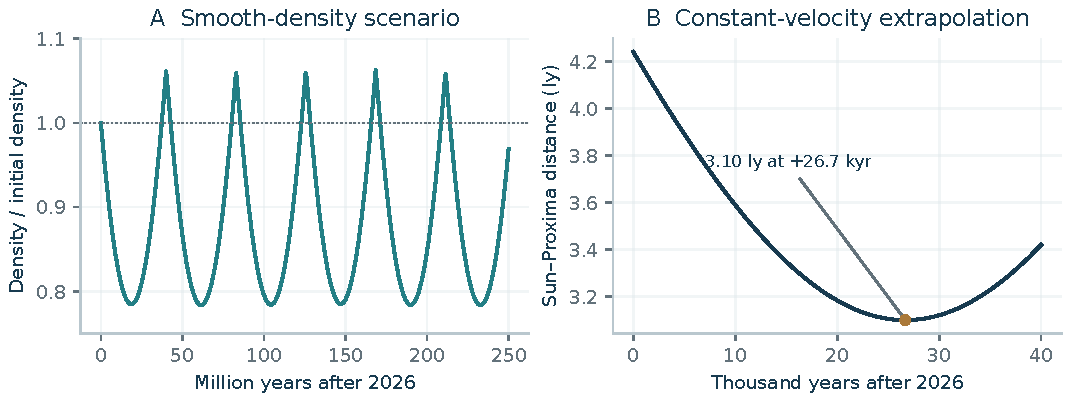
\includegraphics[width=\linewidth,height=68mm,keepaspectratio]{neighbourhood.pdf}\end{center}
\figcap{Two independent models with different clocks. A: adopted smooth-density profile along the Solar orbit. B: constant-velocity Sun--Proxima extrapolation. The apparent minimum in B is not a precision encounter forecast.}

\begin{minipage}[t]{.485\linewidth}\vspace{0pt}\setlength{\parskip}{3pt}
\subsection*{Density is not a discovery count}
A historical census of \ReportDensityLocalStars{} stars within 10 pc [5] sets the local reference:
\[
 n_0=\frac{\ReportDensityLocalStars{}}{(4\pi/3)(10\unit{pc})^3}
     =\ReportDensityLocal\unit{pc^{-3}}.
\]
The adopted thin/thick-disk scenario [6] ranges over \textbf{\ReportDensityMinRatio{}--\ReportDensityMaxRatio{}} times its initial density in 250 Myr: about \textbf{\ReportDensityMinStars{}--\ReportDensityMaxStars{} stars} in an instantaneous 10 pc sphere. It omits spiral-arm enhancements, clusters and migration. These are neither distinct arrivals nor planets found.
\end{minipage}\hfill
\begin{minipage}[t]{.485\linewidth}\vspace{0pt}\setlength{\parskip}{3pt}
\subsection*{Proxima is approaching now}
The adopted historical inputs [7] give about \textbf{\ReportProximaInitial{} ly} in 2026 and a radial velocity of \textbf{$\ReportProximaRadial\unit{km\,s^{-1}}$}; distance is decreasing. The total relative speed is about $\ReportProximaSpeed\unit{km\,s^{-1}}$.

Straight-line propagation gives a minimum near \textbf{\ReportProximaClosest{} ly after \ReportProximaClosestYears{} years}. This omits the Alpha Centauri system's orbital dynamics and Galactic differential acceleration. A negative radial speed today does not imply permanent approach.
\end{minipage}

\subsection*{The next 100, 1,000 and 10,000 years}
\begin{tabularx}{\linewidth}{@{}rXXX@{}}\toprule
Years & Solar path at \ReportSolarSpeed{} km/s & Median sightline shift & Accessibility change\\\midrule
100 & \ReportCenturyTablePath{} ly & \ReportCenturyTableSightline{} arcsec & $\ReportCenturyTableChange\%$\\
1,000 & \ReportMillenniumTablePath{} ly & \ReportMillenniumTableSightline{} arcsec & $\ReportMillenniumTableChange\%$\\
10,000 & \ReportTenMillenniaTablePath{} ly & $\ReportTenMillenniaTableSightline^\circ$ & $\ReportTenMillenniaTableChange\%$\\\bottomrule
\end{tabularx}\par\vspace{7pt}
The last two columns use the same selected \ReportSampleSize{} Gaia sources and baseline imaging thresholds as page 3. They are nominal constant-relative-velocity calculations, with \textbf{no new uncertainty propagation} for the longer intervals. Binary dynamics and differential Galactic acceleration are omitted. The score responds to distance and thresholds, not sky angle alone.

\takeaway{Still local}{In 10,000 years, the model Sun sweeps only $\ReportTenThousandAngle^\circ$ around the Galactic centre. A path of \ReportTenThousandPath{} light-years does not place it in a different spiral arm. Closer targets may be easier to study, but none of these results establishes life or predicts a habitable-planet discovery.}
